\documentclass[11pt]{article}
\usepackage[utf8]{inputenc}
\usepackage[margin=1in]{geometry}
\usepackage{amsmath, amssymb, amsthm}
\usepackage{listings}
\usepackage{color}
\usepackage{tikz}
\usetikzlibrary{matrix,arrows,positioning,calc}

% Code Style Setup
\definecolor{codegreen}{rgb}{0,0.6,0}
\definecolor{codegray}{rgb}{0.5,0.5,0.5}
\definecolor{codepurple}{rgb}{0.58,0,0.82}
\definecolor{backcolor}{rgb}{0.95,0.95,0.92}

\lstset{
    backgroundcolor=\color{backcolor},   
    commentstyle=\color{codegreen},
    keywordstyle=\color{blue},
    numberstyle=\tiny\color{codegray},
    stringstyle=\color{codepurple},
    basicstyle=\ttfamily\small,
    breakatwhitespace=false,         
    breaklines=true,                 
    captionpos=b,                    
    keepspaces=true,                 
    numbers=left,                    
    numbersep=5pt,                  
    showspaces=false,                
    showstringspaces=false,
    showtabs=false,                  
    tabsize=4
}

\title{Homework Assignment 6 \\ \large Concepts of Programming Languages}
\author{Steven Ou}
\date{\today}

\begin{document}

\maketitle
\tableofcontents
\newpage

% ==========================================
% CHAPTER 8
% ==========================================
\section{Chapter 8: Statement-Level Control Structures}

\subsection{Q1: Programming Exercises, Question 1}
\textbf{Question:} Rewrite the following pseudocode segment using a loop structure in the specified languages. For each language, provide both a \texttt{while} loop and a \texttt{for} loop solution[cite: 2]. Assume all variables are integer type[cite: 1]. Discuss which language has the best writability, readability, and the best combination of the two[cite: 1].
\begin{lstlisting}[language=C]
    k = (j + 13) / 27
loop:
    if k > 10 then goto out
    k = k + 1
    i = 3 * k - 1
    goto loop
out: ...
\end{lstlisting}

\noindent\textbf{Solution:}

\subsubsection*{C++/Java - Solution 1: Using a \texttt{while} Loop}
The loop evaluates the condition pre-test style at the top of the structure. As long as $k \le 10$, the block increments $k$ and updates $i$.
\begin{lstlisting}[language=Java]
int k = (j + 13) / 27;
int i = 0; // Assuming initial setup definition

while (k <= 10) {
    k = k + 1;
    i = 3 * k - 1;
}
\end{lstlisting}

\subsubsection*{C++/Java - Solution 2: Using a \texttt{for} Loop}
We can implement the exact same execution logic using a standard \texttt{for} loop configuration. Since $k$ initializes before evaluation and increments immediately inside the body before computing $i$, we can leave the loop update expression slot blank.
\begin{lstlisting}[language=Java]
int i = 0;

for (int k = (j + 13) / 27; k <= 10; ) {
    k = k + 1;
    i = 3 * k - 1;
}
\end{lstlisting}

\subsubsection*{Python - Solution 1: Using a \texttt{while} Loop}
\begin{lstlisting}[language=Python]
k = (j + 13) // 27  # Explicit integer floor division
while k <= 10:
    k += 1
    i = 3 * k - 1
\end{lstlisting}

\subsubsection*{Python - Solution 2: Using a \texttt{for} Loop}
Because Python's standard \texttt{for} loop iterates over a predetermined range or sequence, dynamic updates to the loop variable inside the body do not shift the iteration sequence. Therefore, to precisely replicate the dynamic step logic using a \texttt{for} structure, we iterate over a controlled bounds sequence generated via a \texttt{range} constructor:
\begin{lstlisting}[language=Python]
initial_k = (j + 13) // 27
if initial_k <= 10:
    for k in range(initial_k + 1, 12):
        i = 3 * k - 1
    k = 11 # To match final state of k after loop termination
\end{lstlisting}

\subsubsection*{Ruby - Solution 1: Using a \texttt{while} Loop}
\begin{lstlisting}[language=Ruby]
k = (j + 13) / 27
while k <= 10
  k += 1
  i = 3 * k - 1
end
\end{lstlisting}

\subsubsection*{Ruby - Solution 2: Using a \texttt{for} Loop}
Similar to Python, Ruby's \texttt{for...in} syntax structures block iterations across static object series intervals. We pass a range sequence spanning from our starting step bound up to the logical loop exit value:
\begin{lstlisting}[language=Ruby]
initial_k = (j + 13) / 27
if initial_k <= 10
  for k in (initial_k + 1)..11
    i = 3 * k - 1
  end
end
\end{lstlisting}

\subsubsection*{Language Metrics Evaluation}
\begin{itemize}
    \item \textbf{Readability:} **Python** provides the best layout transparency. Removing unnecessary syntactic symbols (like brackets or block closures) presents clean code lines. However, for this specific problem pattern, the \texttt{while} loop variant reads significantly cleaner across all languages than the forced bounded sequential \texttt{for} mechanisms.
    \item \textbf{Writability:} **Python/Ruby** minimize structural setup steps by dropping strict type definitions, semicolons, and condition block parentheses.
    \item \textbf{Best Combination:} **Python** provides the optimal balance here. Its explicit \texttt{//} floor division operator clarifies integer division handling constraints instantly without requiring context lookups.
\end{itemize}

\subsection{Q2: Programming Exercises, Question 5}
\textbf{Question:} Rubin (1987) uses a code segment finding the first all-zero row of an $n \times n$ matrix to argue that \texttt{goto} statements improve readability. Rewrite this code without \texttt{goto} statements in C, C++, Java, or C\#. Compare the readability of your code to the original example.\\

\noindent\textbf{Solution:}

\subsubsection*{Implementation without gotos (Java variant using boolean flags)}
\begin{lstlisting}[language=Java]
boolean allZeroRowFound = false;
for (int i = 1; i <= n; i++) {
    boolean isZeroRow = true;
    for (int j = 1; j <= n; j++) {
        if (x[i][j] != 0) {
            isZeroRow = false;
            break; // Terminate inner row scanning loop
        }
    }
    if (isZeroRow) {
        System.out.println("First all-zero row is: " + i);
        allZeroRowFound = true;
        break; % Terminate outer row iteration loop
    }
}
\end{lstlisting}

\subsubsection*{Readability Comparison Evaluation}
\begin{itemize}
    \item \textbf{The Original Code (With Goto):} The \texttt{goto reject} bypasses nested execution structures cleanly when a non-zero element is found. However, it breaks structured programming principles by forcing sudden jumps across scope boundaries.
    \item \textbf{The Rewritten Code (Without Goto):} Replacing the jump with explicit control states (\texttt{isZeroRow}) maintains clean structural nesting. It enhances code clarity because loops terminate through conventional control structures (\texttt{break}) instead of unconstrained labels.
\end{itemize}

\newpage
% ==========================================
% CHAPTER 9
% ==========================================
\section{Chapter 9: Subprograms}

\subsection{Q4: Problem Set, Question 5}
\textbf{Question:} Consider the following code segment:
\begin{lstlisting}[language=C]
void swap(int a, int b) {
    int temp;
    temp = a;
    a = b;
    b = temp;
}
void main() {
    int value = 2, list[5] = {1, 3, 5, 7, 9};
    swap(value, list[0]);
    swap(list[0], list[1]);
    swap(value, list[value]);
}
\end{lstlisting}
Trace the variable updates across all three individual calls to \texttt{swap}.\\

\noindent\textbf{Solution:}

\subsubsection*{a. Passed by Value}
Formal copies are local to the subprogram scope and do not propagate mutations back to the caller frame on termination.
\begin{itemize}
    \item \textbf{Initial state}: \texttt{value = 2}, \texttt{list = [1, 3, 5, 7, 9]}
    \item \textbf{Call 1} \texttt{swap(2, 1)}: Mutates local variables only. No changes in \texttt{main}.
    \item \textbf{Call 2} \texttt{swap(1, 3)}: Mutates local variables only. No changes in \texttt{main}.
    \item \textbf{Call 3} \texttt{swap(2, 5)}: Mutates local variables only. No changes in \texttt{main}.
    \item \textbf{Final state}: \texttt{value = 2}, \texttt{list = [1, 3, 5, 7, 9]}
\end{itemize}

\subsubsection*{b. Passed by Reference}
Formal parameters act as live reference pointers bound directly to the actual arguments' memory addresses.
\begin{itemize}
    \item \textbf{Initial state}: \texttt{value = 2}, \texttt{list = [1, 3, 5, 7, 9]}
    \item \textbf{Call 1} \texttt{swap(value, list[0])}: References point to \texttt{value} and \texttt{list[0]}. Swapping them swaps their values in \texttt{main}.
          \\ State changes to: \texttt{value = 1}, \texttt{list = [2, 3, 5, 7, 9]}
    \item \textbf{Call 2} \texttt{swap(list[0], list[1])}: References point to \texttt{list[0]} (currently 2) and \texttt{list[1]} (3).
          \\ State changes to: \texttt{value = 1}, \texttt{list = [3, 2, 5, 7, 9]}
    \item \textbf{Call 3} \texttt{swap(value, list[value])}: References point to \texttt{value} (currently 1) and \texttt{list[1]} (currently 2).
          \\ State changes to: \texttt{value = 2}, \texttt{list = [3, 1, 5, 7, 9]}
\end{itemize}

\subsubsection*{c. Passed by Value-Result}
Values are copied into local variables at the call site, and their final local values are copied back to the caller's arguments upon subprogram termination.
\begin{itemize}
    \item \textbf{Call 1}: Copies \texttt{a = value = 2} and \texttt{b = list[0] = 1}. After local swap, \texttt{a = 1, b = 2}. On return, these values are written back to their respective arguments.
          \\ State changes to: \texttt{value = 1}, \texttt{list = [2, 3, 5, 7, 9]}
    \item \textbf{Call 2}: Copies \texttt{a = list[0] = 2} and \texttt{b = list[1] = 3}. After local swap, \texttt{a = 3, b = 2}. On return, these values are written back to their respective arguments.
          \\ State changes to: \texttt{value = 1}, \texttt{list = [3, 2, 5, 7, 9]}
    \item \textbf{Call 3}: Actual parameters are evaluated at the call site. The address for \texttt{list[value]} resolves to \texttt{list[1]} because \texttt{value} is 1. Copies \texttt{a = value = 1} and \texttt{b = list[1] = 2}. After local swap, \texttt{a = 2, b = 1}. On return, these values are copied back to their corresponding variables.
          \\ State changes to: \texttt{value = 2}, \texttt{list = [3, 1, 5, 7, 9]}
\end{itemize}

\subsection{Q5: Problem Set, Question 7}
\textbf{Question:} Consider the following program written in C syntax:
\begin{lstlisting}[language=C]
void fun(int first, int second) {
    first += first;
    second += second;
}
void main() {
    int list[2] = {1, 3};
    fun(list[0], list[1]);
}
\end{lstlisting}
Determine the final values of the \texttt{list} array under the three parameter passing models.\\

\noindent\textbf{Solution:}
\begin{itemize}
    \item \textbf{a. Passed by value:} Operations occur within local scopes, leaving caller variables unaffected. \\ Final values: \texttt{list[0] = 1}, \texttt{list[1] = 3}
    \item \textbf{b. Passed by reference:} Subprogram updates directly modify the caller's arguments via pointer bindings. \\ Final values: \texttt{list[0] = 2}, \texttt{list[1] = 6}
    \item \textbf{c. Passed by value-result:} Initial values are copied into local parameters, doubled locally, and then copied back into the caller's array slots upon function return. \\ Final values: \texttt{list[0] = 2}, \texttt{list[1] = 6}
\end{itemize}

\newpage
% ==========================================
% CHAPTER 10
% ==========================================
\section{Chapter 10: Implementing Subprograms}

\subsection{Q6, Q7, Q8: Activation Records Trace (Problem Set 1, 2, 3)}
\textbf{Trace Scenario:} The program sequence moves through the execution chain: \texttt{bigsub} calls \texttt{a}, \texttt{a} calls \texttt{b}, \texttt{b} calls \texttt{a}, \texttt{a} calls \texttt{c}, and \texttt{c} calls \texttt{d}.

\begin{figure}[h!]
\centering
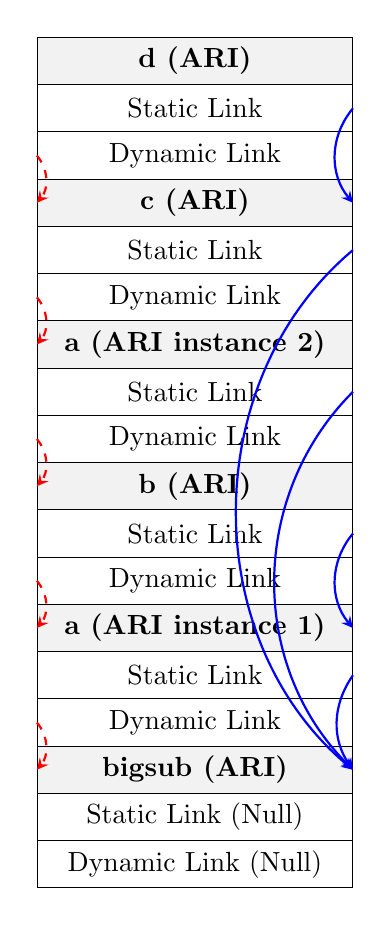
\begin{tikzpicture}[
    stack/.style={matrix of nodes, nodes={draw, minimum width=4cm, minimum height=0.6cm, anchor=center}, column sep=0pt, row sep=-\pgflinewidth},
    link/.style={->,>=stealth,thick}
]

\matrix [stack] (ari) {
    |[fill=gray!10]| \textbf{d (ARI)} \\
    Static Link \\
    Dynamic Link \\
    |[fill=gray!10]| \textbf{c (ARI)} \\
    Static Link \\
    Dynamic Link \\
    |[fill=gray!10]| \textbf{a (ARI instance 2)} \\
    Static Link \\
    Dynamic Link \\
    |[fill=gray!10]| \textbf{b (ARI)} \\
    Static Link \\
    Dynamic Link \\
    |[fill=gray!10]| \textbf{a (ARI instance 1)} \\
    Static Link \\
    Dynamic Link \\
    |[fill=gray!10]| \textbf{bigsub (ARI)} \\
    Static Link (Null) \\
    Dynamic Link (Null) \\
};

% Dynamic Links (dashed red, tracking immediate callers)
\draw[link, red, dashed, bend left=40] (ari-3-1.west) to (ari-4-1.west);
\draw[link, red, dashed, bend left=40] (ari-6-1.west) to (ari-7-1.west);
\draw[link, red, dashed, bend left=40] (ari-9-1.west) to (ari-10-1.west);
\draw[link, red, dashed, bend left=40] (ari-12-1.west) to (ari-13-1.west);
\draw[link, red, dashed, bend left=40] (ari-15-1.west) to (ari-16-1.west);

% Static Links (solid blue, tracking lexical parents)
\draw[link, blue, bend right=40] (ari-2-1.east) to (ari-4-1.east);   % d points to c
\draw[link, blue, bend right=50] (ari-5-1.east) to (ari-16-1.east);  % c points to bigsub
\draw[link, blue, bend right=45] (ari-8-1.east) to (ari-16-1.east);  % a2 points to bigsub
\draw[link, blue, bend right=40] (ari-11-1.east) to (ari-13-1.east); % b points to a1
\draw[link, blue, bend right=35] (ari-14-1.east) to (ari-16-1.east); % a1 points to bigsub

\end{tikzpicture}
\caption{Stack frame diagram illustrating static and dynamic link paths when execution reaches \texttt{d}.}
\end{figure}

\subsection{Q9: Problem Set, Question 4}
\textbf{Question:} Show the stack with all activation record instances, including static and dynamic chains, when execution reaches position 1 under deep-access dynamic scoping layout environments.\\

\noindent\textbf{Solution:}
Deep-access scoping implements variable searches by traversing the dynamic link chain backward through active stack frames until the matching variable name identifier is found.

\begin{figure}[h!]
\centering
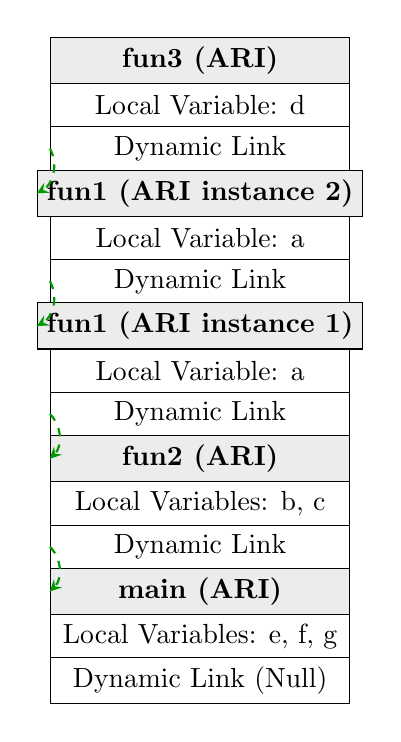
\begin{tikzpicture}[
    stack/.style={matrix of nodes, nodes={draw, minimum width=3.8cm, minimum height=0.55cm, anchor=center}, column sep=0pt, row sep=-\pgflinewidth},
    link/.style={->,>=stealth,thick,green!60!black}
]

\matrix [stack] (deepstack) {
    |[fill=gray!15]| \textbf{fun3 (ARI)} \\
    Local Variable: d \\
    Dynamic Link \\
    |[fill=gray!15]| \textbf{fun1 (ARI instance 2)} \\
    Local Variable: a \\
    Dynamic Link \\
    |[fill=gray!15]| \textbf{fun1 (ARI instance 1)} \\
    Local Variable: a \\
    Dynamic Link \\
    |[fill=gray!15]| \textbf{fun2 (ARI)} \\
    Local Variables: b, c \\
    Dynamic Link \\
    |[fill=gray!15]| \textbf{main (ARI)} \\
    Local Variables: e, f, g \\
    Dynamic Link (Null) \\
};

% Trace Arrows
\draw[link, dashed, bend left=45] (deepstack-3-1.west) to (deepstack-4-1.west);
\draw[link, dashed, bend left=45] (deepstack-6-1.west) to (deepstack-7-1.west);
\draw[link, dashed, bend left=45] (deepstack-9-1.west) to (deepstack-10-1.west);
\draw[link, dashed, bend left=45] (deepstack-12-1.west) to (deepstack-13-1.west);

\end{tikzpicture}
\caption{Dynamic scoping call trace hierarchy using deep-access mechanics.}
\end{figure}

\subsection{Q10: Problem Set, Question 5}
\textbf{Question:} Show the state configuration layout maps for Problem 4 assuming a shallow-access runtime model environment design layout.\\

\noindent\textbf{Solution:}
Shallow-access scoping maps each variable name identifier to its own independent global variable runtime tracking stack. This layout provides fast $O(1)$ lookup times.

\begin{figure}[h!]
\centering
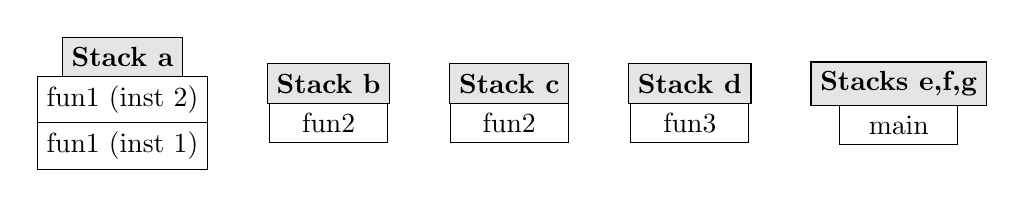
\begin{tikzpicture}[
    vstack/.style={matrix of nodes, nodes={draw, minimum width=1.5cm, minimum height=0.5cm, anchor=center}, column sep=0pt, row sep=-\pgflinewidth},
    title/.style={font=\bfseries\small, depth=0ex, bottom color=gray!30, top color=gray!10}
]

\matrix [vstack] (stackA) {
    |[fill=gray!20]| \textbf{Stack a} \\ fun1 (inst 2) \\ fun1 (inst 1) \\
};
\matrix [vstack, right=0.5cm of stackA] (stackB) {
    |[fill=gray!20]| \textbf{Stack b} \\ fun2 \\
};
\matrix [vstack, right=0.5cm of stackB] (stackC) {
    |[fill=gray!20]| \textbf{Stack c} \\ fun2 \\
};
\matrix [vstack, right=0.5cm of stackC] (stackD) {
    |[fill=gray!20]| \textbf{Stack d} \\ fun3 \\
};
\matrix [vstack, right=0.5cm of stackD] (stackEFG) {
    |[fill=gray!20]| \textbf{Stacks e,f,g} \\ main \\
};

\end{tikzpicture}
\caption{Shallow-access structure maps isolated global stacks for each active identifier.}
\end{figure}

\newpage
% ==========================================
% CHAPTER 15
% ==========================================
\section{Chapter 15: Functional Programming Languages}

\subsection{Q11: Programming Exercises, Question 2}
\textbf{Question:} Write a Scheme function that computes the real roots of a given quadratic equation using an \texttt{if} function block.

\begin{lstlisting}[language=Lisp]
(define (quadratic-roots a b c)
  (let ((disc (- (* b b) (* 4 a c))))
    (if (< disc 0)
        "Complex roots encountered"
        (list (/ (+ (- b) (sqrt disc)) (* 2 a))
              (/ (- (- b) (sqrt disc)) (* 2 a))))))
\end{lstlisting}

\subsubsection*{Verification Execution Traces}
\begin{itemize}
    \item \texttt{(quadratic-roots 1 -5 6)} $\rightarrow$ Returns \texttt{'(3.0 2.0)}
    \item \texttt{(quadratic-roots 1 2 5)} $\rightarrow$ Returns \texttt{"Complex roots encountered"}
\end{itemize}

\subsection{Q12: Programming Exercises, Question 5}
\textbf{Question:} Write a Scheme function that returns the number of zeros in a given simple list of numbers.

\begin{lstlisting}[language=Lisp]
(define (count-zeros lis)
  (cond
    ((null? lis) 0)
    ((= (car lis) 0) (+ 1 (count-zeros (cdr lis))))
    (else (count-zeros (cdr lis)))))
\end{lstlisting}

\subsubsection*{Verification Execution Traces}
\begin{itemize}
    \item \texttt{(count-zeros '(0 1 2 0 3 0))} $\rightarrow$ Returns \texttt{3}
    \item \texttt{(count-zeros '(1 2 3 4))} $\rightarrow$ Returns \texttt{0}
\end{itemize}

\subsection{Q13: Programming Exercises, Question 11}
\textbf{Question:} Write a Scheme function that returns the reverse of its simple list parameter.

\begin{lstlisting}[language=Lisp]
(define (reverse-simple-list lis)
  (define (rev-helper rem acc)
    (if (null? rem)
        acc
        (rev-helper (cdr rem) (cons (car rem) acc))))
  (rev-helper lis '()))
\end{lstlisting}

\subsubsection*{Verification Execution Traces}
\begin{itemize}
    \item \texttt{(reverse-simple-list '(a b c d))} $\rightarrow$ Returns \texttt{'(d c b a)}
    \item \texttt{(reverse-simple-list '(1))} $\rightarrow$ Returns \texttt{'(1)}
\end{itemize}

\subsection{Q14: Programming Exercises, Question 13}
\textbf{Question:} Write a Scheme function that returns the union of two simple list parameters that represent sets (containing only unique items).
\begin{lstlisting}[language=Lisp]
(define (set-union set1 set2)
  (cond
    ((null? set1) set2)
    ((member (car set1) set2) (set-union (cdr set1) set2))
    (else (cons (car set1) (set-union (cdr set1) set2)))))
\end{lstlisting}

\subsubsection*{Verification Execution Traces}
\begin{itemize}
    \item \texttt{(set-union '(1 2 3) '(3 4 5))} $\rightarrow$ Returns \texttt{'(1 2 3 4 5)}
    \item \texttt{(set-union '(a b) '(c d))} $\rightarrow$ Returns \texttt{'(a b c d)}
\end{itemize}

\subsection{Q15: Programming Exercises, Question 16}
\textbf{Question:} Write a Scheme function that takes a simple list of numbers as its parameter and returns a list identical to the parameter list except with the numbers in ascending order.

\begin{lstlisting}[language=Lisp]
(define (insert num sorted-lis)
  (cond
    ((null? sorted-lis) (list num))
    ((<= num (car sorted-lis)) (cons num sorted-lis))
    (else (cons (car sorted-lis) (insert num (cdr sorted-lis))))))

(define (insertion-sort lis)
  (if (null? lis)
      '()
      (insert (car lis) (insertion-sort (cdr lis)))))
\end{lstlisting}

\subsubsection*{Verification Execution Traces}
\begin{itemize}
    \item \texttt{(insertion-sort '(5 2 9 1 3))} $\rightarrow$ Returns \texttt{'(1 2 3 5 9)}
    \item \texttt{(insertion-sort '(10 -2 4 0))} $\rightarrow$ Returns \texttt{'(-2 0 4 10)}
\end{itemize}

\end{document}